%!TEX root = ../vernier.tex
\chapter{Visualization} \label{sec:visualization}

Discussions that relate image perception and cognitive understanding can be traced as far back as the early Greek philosophers. Socrates considered that sensory experiences create images in the human mind, regarded as mental representations of the real world. Around 350BC, Aristoteles stated that "thought is impossible without an image".

\citet{ref:gershon94} defines visualization as follows: "Visualization is more than a method of computing. Visualization is the process of transforming information into a visual form, enabling users to observe the information. The resulting visual display enables the scientist or engineer to perceive visually features which are hidden in the data but nevertheless are needed for data exploration and analysis."

The resulting visual representation can be used to both to confirm the known, (i.e. validating the fit a given model with a dataset) and discovering the unknown (i.e. creating insight that supports a new model in the data). But first, we need first to recognize when visualization is actually useful. As questioned by Telea%TODO {link to scivis slides}
, if a question can be answered by a compact, precise query (e.g. what is most complex class in a given package), why visualize? Or if a decision can be automated, why put a human in the process? (e.g. decide which classes are considered \textit{dead code} and should be removed from a project.)

%TODO: improve this part later
Visualization be can useful in many applications. For example, when there's too much data and we don't have time to analyze or make sense of it all, allowing for a overview of the data's features. It is useful to get insight about distribution, correlations, behavior, and relationships. It can also be useful to answer qualitative and complex questions. Lastly, it is fundamental for communication.

The challenge of creating a good visualization lies in tailoring visual representations that objectively communicate features of the data. When our representations are not suitable, as recognized by van Vijk on figure \ref{fig:botanic}, visualization might not be very helpful. Bad representations might also lead to a visual result that is in misalignment with the original data, and as stated by Edward Tufte, "clutter and confusion are failures of design, not attributes of information".

\begin{figure}[h]
	\centering
	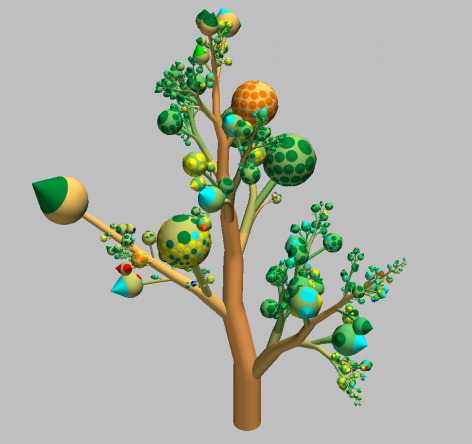
\includegraphics[width=0.7\textwidth]{figures/botanic.png}
	\caption {van Wijk questions: "Botanic visualization contents of a hard disk. Useful or just a nice picture?"}
	\label{fig:botanic}
  %TODO add ref
\end{figure}

The dataset we are trying to understand (illustrated as A on Figure \ref{fig:data_pipeline}) is a set of $R$ revisions where each revision $r_{t}$ $\in$ [$r_{s}, r_{e}$] \hspace{0.2cm}is a set of entities $E = \{ e_{i}\}$ $\subset$ $\mathbb{R}^{n}$ that portray a feature vector of $n = 43$ real-valued quality metrics of a given software class.

For each revision $r_{t}$ $\in$ \lbrack  $r_{s}, r_{e}$\rbrack, a dimensionality reduction technique is used to generate a 2D projection $P_{t} = \{q_{i} \} \subset{\mathbb{R}^{2}}$ where $i$ is the number of observations and $q$ a point in 2D space. The projection set $P$ depicts the class similarity throughout the project's history and is illustrated as B on Figure \ref{fig:data_pipeline}. More details on the technique are present on Section \ref{sec:proj}.

Once we have collected the two time-dependent datasets, we must develop a tool to visualize it. In this chapter we will discuss our attempts in transforming this complex data into visual forms that allow for insightful answers. To develop these techniques no libraries were used apart from OpenGL for the rendering and GLUT/GLUI for the window/GUI management. The source code is available at \url{https://github.com/EduardoVernier/metric-view} and from now on, we will address the visualization tool as MetricView.
